\section{Results}\label{sec_results}

    In the first step of this experiment, the pressure sensor has to be calibrated at known pressures and temperatures.
    The result of this calibration is presented in Fig.~\ref{fig_calibration}

    \begin{figure}[H]
        \centering
        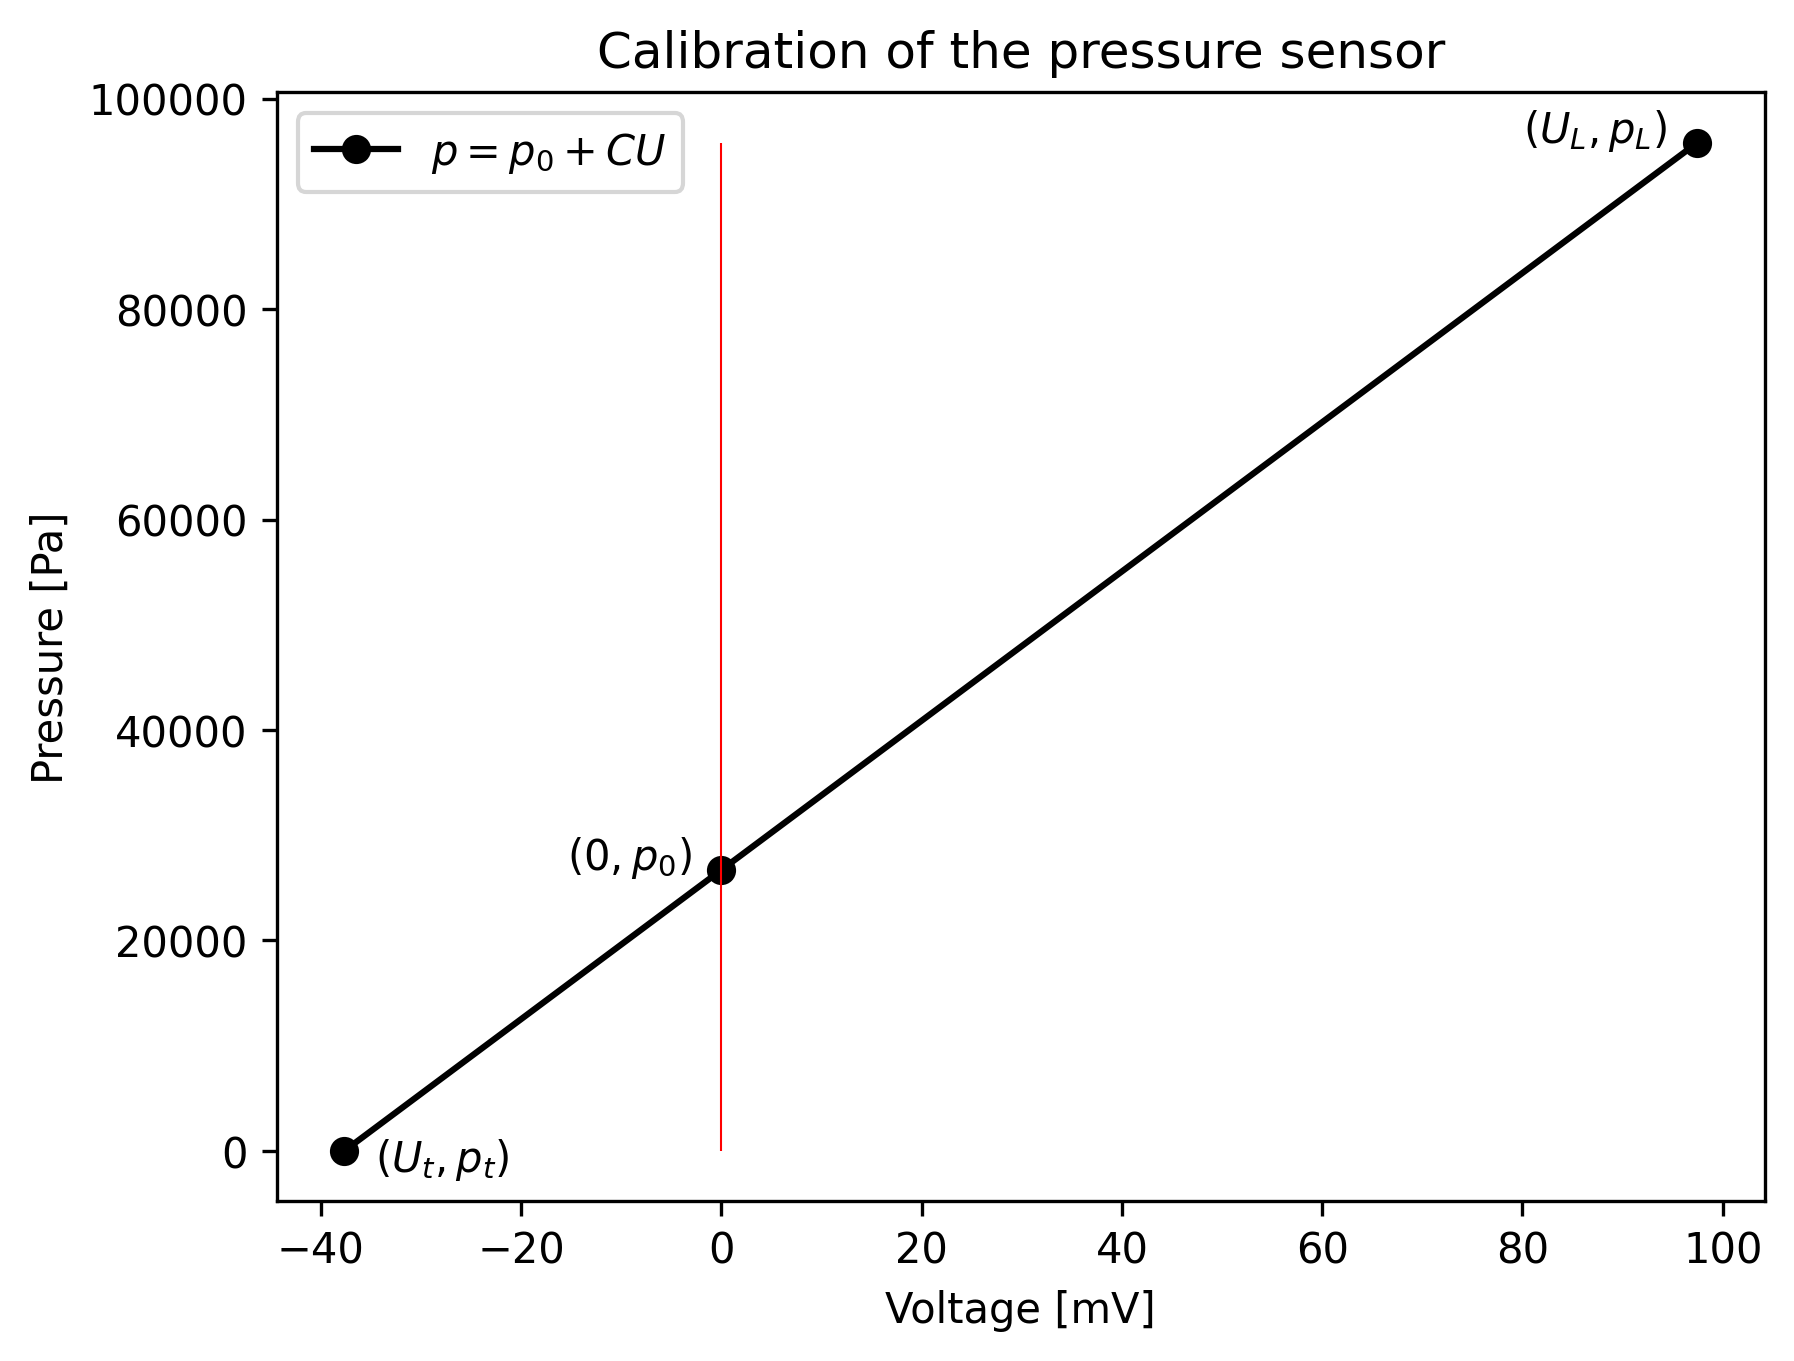
\includegraphics[]{src/images/calibration.png}
        \caption{Calibration of the pressure sensor: A linear fit through $(U_L,p_L)$ and $(U_t,p_t)$ determines the slope $C$. $p_0$ shows the y-intersect at voltage $U_0 = 0$}
        \label{fig_calibration}
    \end{figure}

    Eq.~\ref{eq_c} is used to calculate the slope of this curve. $p_0$ can then be found by entering a pair of known values into eq.~\ref{eq_p0}, such as $(U_t,p_t)$.
    \begin{align}
        C &= \frac{p_L - p_t}{U_L - U_t} \label{eq_c}\\
        p_0 &= p_t - C U_t \label{eq_p0}
    \end{align}

    Using the slope $C$ and y-offset $p_0$, which we determined in this first step, we can calculate the pressure
    of any sensor reading using formula \ref{eq_pressure}.

    \begin{align}
        p(U) = p_0 + CU \label{eq_pressure}
    \end{align}

    To determine the uncertainties in eq.~\ref{eq_pressure}, we first have to calculate the errors in $p_0$, $C$ and $U$.
    Using the gaussian error propagation, we can then determine the error of the entire equation.


    From the manufacturer's datasheet, we know that the linearity of the sensor is guaranteed up to $\pm 0.05\%$ full scale. % of the full scale?
    This means that the sensor signal error is at most $0.05\%$ of $150\si{\milli\volt}$, thus $0.075\si{\milli\volt}$.

    Furthermore, it has to be taken into account, that the temperature of the sensor may vary from when
    it was calibrated and when the measurement was made. We can assume a voltage difference of $\pm 0.08\si{\milli\volt}/\si{\celsius}$ at $p = 0$.
    The slope of this curve can vary by $\pm 0.1\% \si{\celsius}$
    This is the uncertainty calculation for $\Delta U$:
    \begin{align}
        \Delta U &= 0.075 \si{\milli\volt} + 0.08 \frac{\si{\milli\volt}}{1 \si{\celsius} \pm 0.1 \% \si{\celsius}}\\
        &= 0.075 \si{\milli\volt} + 0.08 \si{\milli\volt} + 8 \cdot 10^{-5} \si{\milli\volt} \label{eq_dlta_u}\\
        \bf \Delta U &= \bf \pm 0.16 ~\si{\bf\milli\volt} \label{dlta_u}
    \end{align}

    The errors in eq.~\ref{eq_dlta_u} were calculated using the gaussian error propagation. Please refer to our jupyter notebook \cite{GitHub}, 
    for the full calculations of all the values and error propagations presented in this chapter.   %LINK GITHUB !!!!

    $\Delta C$ can be determined in a similar way, based on eq.~\ref{eq_c}:
    \begin{align}
        \Delta C &= \sqrt{ \left(\frac{\partial C}{\partial p_L} \Delta p_L \right)^2 +
                        \left(\frac{\partial C}{\partial p_t} \Delta p_t \right)^2 +
                        \left(\frac{\partial C}{\partial U_L} \Delta U_L \right)^2 +
                        \left(\frac{\partial C}{\partial U_t} \Delta U_t \right)^2 } \label{eq_dlta_c}
    \end{align}

    Using the errors for $U$ determined in eq. \ref{dlta_u}, as well as $\Delta p_t = \pm 0.1 \si{\milli\bar}$ given in the manual and $\Delta p_L = 200~\si{\pascal}$,
    we can determine a value for $\Delta C$ using eq.~\ref{eq_dlta_c}:
    \begin{align}
        \Delta C &= \pm 1.878 \label{dlta_c}\\
        \bf C &= \bf 709 \pm 2
    \end{align}

    Lastly, we have to determine the error for $\Delta p_0$. The error can be calculated in the same way as before, based on equation \ref{eq_p0}.
    Due to the fact that the calculated sensor error $\Delta U$ is full scale, it can be assumed for all sensor readings $U_i$.
    \begin{align}
        \Delta p_0 &= \sqrt{ \left(\frac{\partial p_0}{\partial C} \Delta C \right)^2 +
                            \left(\frac{\partial p_0}{\partial U_t} \Delta U_t \right)^2 +
                            \Delta p_t^2}\\
        \Delta p_0 &= \pm 131 ~\si{\pascal} \label{dlta_p0}\\
        \bf p_0 &= \bf (26.7 \pm 0.1) ~\si{\bf\kilo\pascal}
    \end{align}

    We now have all the values for calculating $\Delta p(U)$. Based on eq. \ref{eq_pressure} we can determine the following error propagation:
    \begin{align}
        \Delta p(U) &= \sqrt{ \left(\frac{\partial p}{\partial C} \Delta C \right)^2 +
                            \left(\frac{\partial p}{\partial U} \Delta U \right)^2 +
                            \Delta p_0^2}\\
        &= \sqrt{ \left( U \Delta C \right)^2 +
                \left( C \Delta U \right)^2 + 
                \Delta p_0^2} \label{eq_dlta_p}
    \end{align}

    \begin{figure}[H]
        \centering
        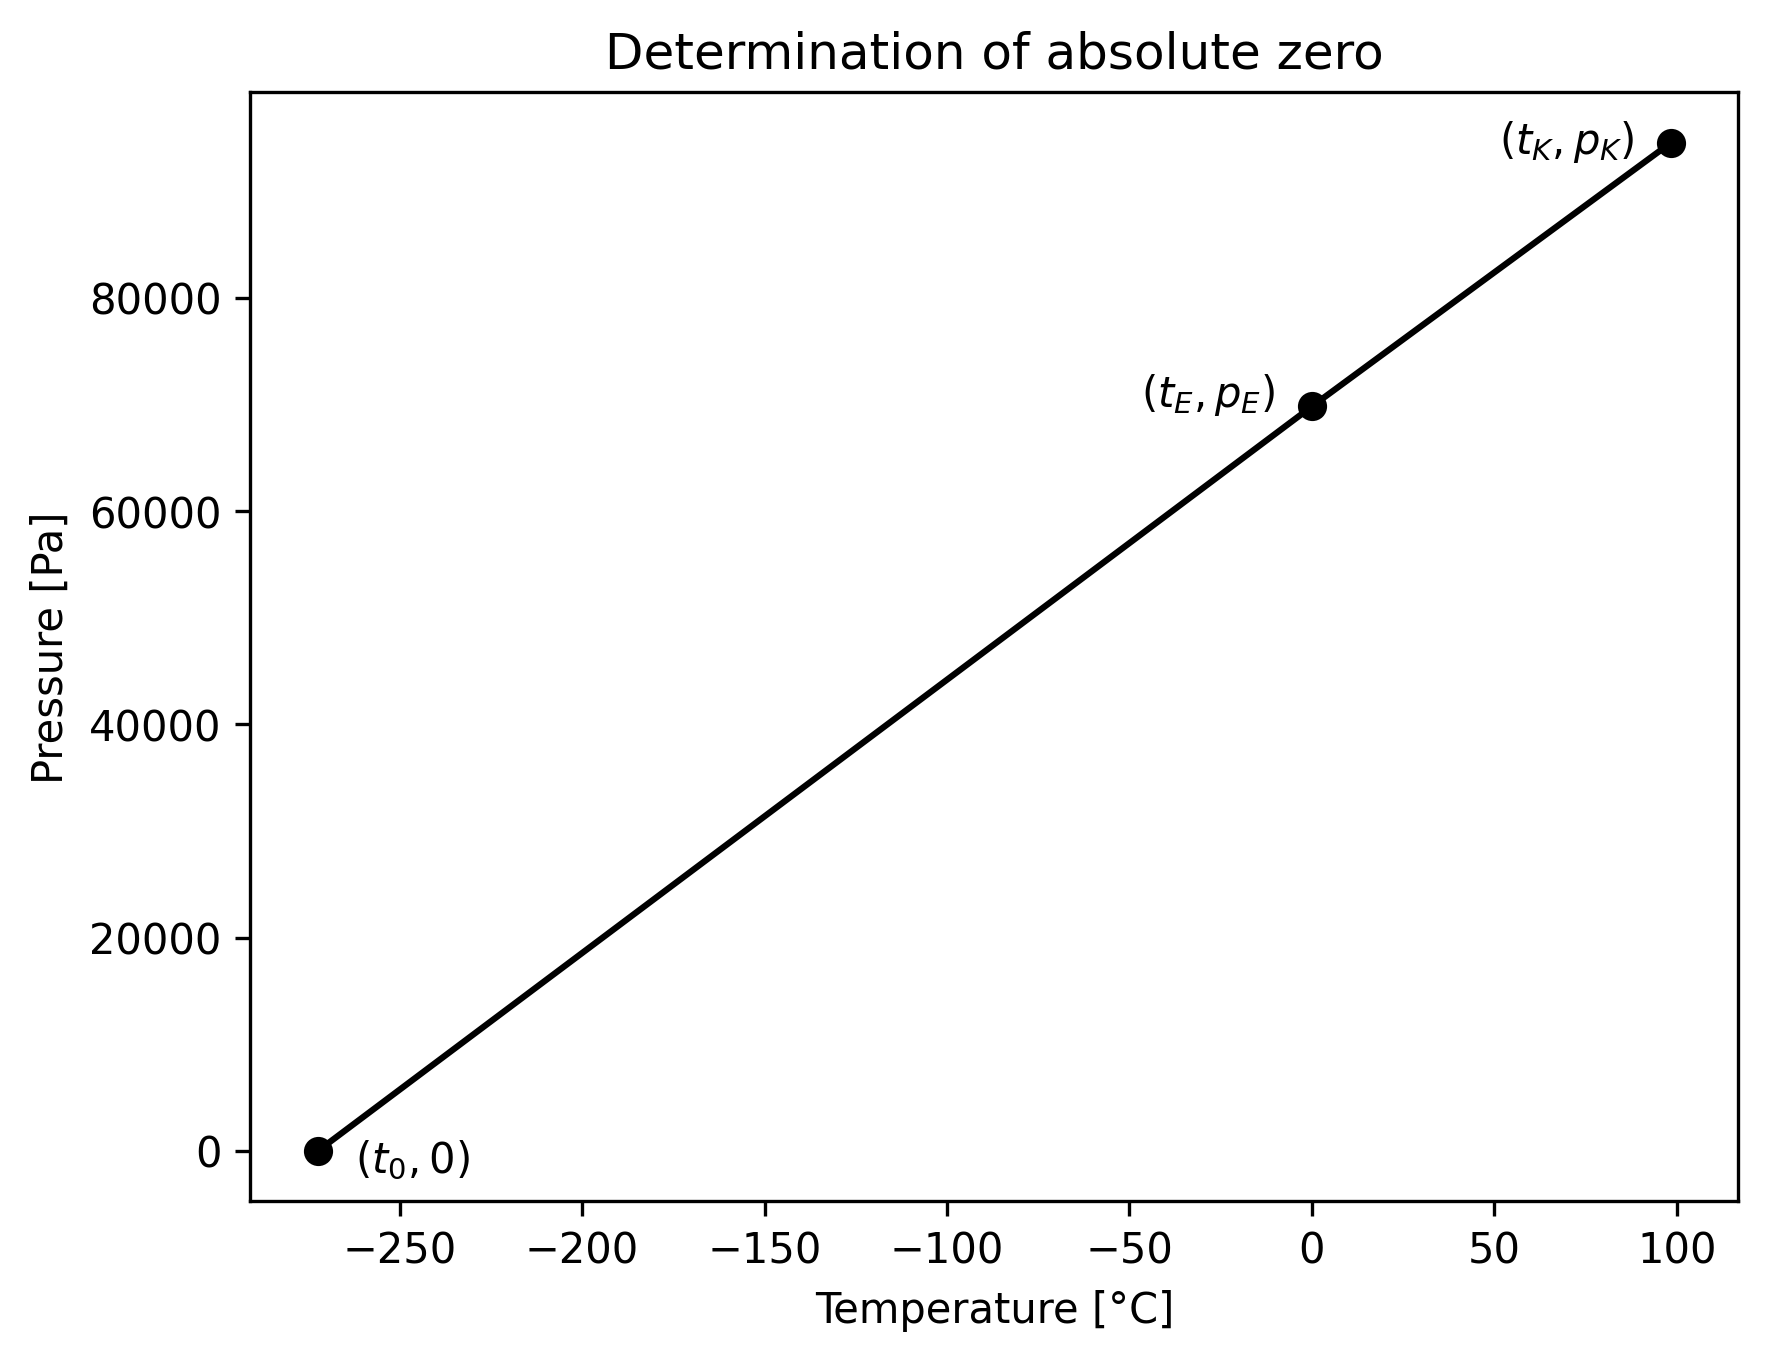
\includegraphics[]{src/images/absolute_zero.png}
        \caption{Determination of absolute zero: Linear fit through $(t_E, p_E)$ and $(t_K, p_K)$ until $p = 0$ is reached.}
        \label{fig_abs_zero}
    \end{figure}
    Fig.~\ref{fig_abs_zero} is a visual representation of how the value for $t_0$ was obtained. Measuring the pressure of the Helium gas at two precisely
    defined temperatures will give us two points on a temperature/pressure graph. The y-intersection of the linear fit through these points will give us an approximative value for $t_0$.
    To get a more precise value, we have to take into account multiple factors like the expansion of the glass bulb under temperature changes, 
    as well as the influence of unevenly heated gas in the connecting tube between the bulb and the sensor.

    In this following paragraph the results from the determination of absolute zero are presented.
    Using eq.~\ref{eq_pressure} the resulting pressures were calculated from the raw sensor data.
    With the derived eq.~\ref{eq_dlta_p} we can then calculate the errors $\Delta p_K, \Delta p_E$. %With the equation derived in eqref...?
    \begin{align}
        p(U_E) &= (69.8 \pm 0.2) ~\si{\kilo\pascal} \label{val_pE}\\
        p(U_K) &= (94.5 \pm 0.2) ~\si{\kilo\pascal} \label{val_pK}
    \end{align}

    As described above the exact value for $t_0$ has to take into account the remaining gas
    in the tube connecting the bulb with the sensor, as well as the thermal expansion of the
    bulb itself. The following quadratic equation calculates the final value for $t_0$ while
    taking into account the factors stated above.
    \begin{align}
        a &= (1 + \varepsilon)p_E - (1 + \epsilon + \gamma t_K)p_K\\
        b &= \varepsilon(p_K - p_E)t_K + (1 + \gamma t_K)p_K t_L - p_E(t_L + t_K)\\
        c &= p_E t_L t_K\\
        t_0 &= \frac{-b \pm \sqrt{b^2 - 4a c}}{2a} \label{eq_t0}
    \end{align}

    Using a barometer in the lab we determined the boiling point of water to be $t_K = 98.323 \si{\celsius}$.
    The temperature in the lab was $t_L = 24 \si{\celsius}$.
    When entering the results from eq.~\ref{val_pE} and~\ref{val_pK}, as well as $t_K$ and $t_L$ into eq.~\ref{eq_t0},
    we get the following result for $t_0$:
    \begin{align}
        t_0 = -275.9~\si{\celsius} \label{val_t0}
    \end{align}

    The error calculation for $t_0$ was again accomplished using the gaussian error propagation.
    Due to the fact that $t_E$, as well as $t_K$, could be determined very precisely, we did not take
    the uncertainties of these values into account in the following error calculation.
    Therefore the only variables whose error margins were considered are $p_E$, as well as $p_K$. % ... whose error margins were considered are...
    \begin{align}
        \Delta t_0 &= \sqrt{ \left(\frac{\partial t_0}{\partial p_E} \Delta p_E \right)^2 +
                            \left(\frac{\partial t_0}{\partial p_K} \Delta p_K \right)^2 }\\
        \Delta t_0 &= \pm 3.53~\si{\celsius} \label{dlta_t0}\\
        \bf t_0 &= \bf (-276 \pm 4)~\si{\bf\celsius} \label{res_t0}
    \end{align}

    In the last part of the experiment, the apparatus was used as a thermometer, to determine the 
    temperature of liquid nitrogen.
    Using eq.~\ref{eq_pressure} the pressure $p_N$ was calculated from the raw sensor data $U_N$.
    \begin{align}
        p_N = 19.6~\si{\kilo\pascal}
    \end{align}

    To calculate the temperature of liquid nitrogen we can use our known value of $t_0$ and solve
    the following equation for $t'_{LN2}$. This will only give us an approximate value, by simply solving a linear approach.
    \begin{align}
        \frac{p_E}{t_E - t_0} \approx& \; \frac{p_N}{t'_{LN2} - t_0}\\
        t'_{LN2} \approx& \; \frac{p_N}{p_E}(t_E - t_0) + t_0
    \end{align}

    Here we again have to take the volume of gas in the tube connecting the bulb with sensor,
    as well as the shrinkage of the glass bulb due to the temperature change into account.
    The following equation will give us an exact value for $t_{LN2}$:
    \begin{align}
        A \equiv& \; \frac{p_E}{t_E - t_0} + \frac{\varepsilon(p_E - p_N)}{t_L - t_0}\\
        =& \; 253.14~\si{\pascal/\celsius}\\
        t_{LN2} =& \; \frac{A t_0 + p_N}{A - \gamma p_N}\\
        =& \; -198.5~\si{\celsius} \label{val_tN}
    \end{align}

    Using the gaussian error propagation the uncertainty for $t_{LN2}$ was calculated. As stated above
    the uncertainties for the variables $t_L$ and $t_E$ are not considered in this calculation either.
    \begin{align}
        \Delta A =& \; \sqrt{ \left(\frac{\partial A}{\partial p_E} \Delta p_E \right)^2 +
                            \left(\frac{\partial A}{\partial p_N} \Delta p_N \right)^2 +
                            \left(\frac{\partial A}{\partial t_0} \Delta t_0 \right)^2 }\\
        =& \; 3.33~\si{\pascal/\celsius}\\
        \Delta t_{LN2} =& \; \sqrt{ \left(\frac{\partial t_{LN2}}{\partial A} \Delta A \right)^2 +
                                    \left(\frac{\partial t_{LN2}}{\partial t_0} \Delta t_0 \right)^2 +
                                    \left(\frac{\partial t_{LN2}}{\partial p_N} \Delta p_N \right)^2 }\\
        =& \; 3.74~\si{\celsius}\\
        \bf t_{LN2} =& \; \bf (-199 \pm 4) ~\si{\bf\celsius} \label{res_tN}
    \end{align}